\chapter{Ανάπτυξη Διαδικτυακής Εφαρμογής iBoot}
Σε αυτό το κεφάλαιο, αναλύονται οι λειτουργίες που παρέχει η διαδικτυακή εφαρμογή στους χρήστες της μέσω Διεπαφής Χρήστη (User Interface) και παρέχεται επεξήγηση των αρχείων κώδικα, ο οποίος συντέλεσε στη δημιουργία του πληροφοριακού συστήματος. Ανάλογα με τον ρόλο του χρήστη που συνδέεται στην εφαρμογή, παρέχονται και οι αντίστοιχες λειτουργίες. Η εμφάνιση της εφαρμογής έχει ίδια αισθητικά χαρακτηριστικά για κάθε είδος χρήστη. Το User Interface θεωρείται από τα πιο σημαντικά μέρη μιας διαδικτυακής εφαρμογής καθώς, αν είναι σχεδιασμένο σωστά, ώστε να είναι εύχρηστο και διαισθητικό, κάνει εύκολη τη χρήση των λειτουργιών του συστήματος, ακόμη και σε χρήστες που πιθανώς δεν είναι εξειδικευμένοι στον τομέα της πληροφορικής.

Για την κατασκευή του User Interface, χρησιμοποιήθηκε η αρχή του Reactive Programming, δηλαδή της μεθόδου προγραμματισμού ιστού ώστε το περιεχόμενο της εφαρμογής να ανανεώνεται δυναμικά και ασύγχρονα με τις ενέργειες του χρήστη, σε ένα εν γένει στατικό περιβάλλον. Όσον αφορά το σχεδιασμό του γραφικού περιβάλλοντος, χρησιμοποιήθηκε Responsive Design, ώστε η εφαρμογή να έχει ομοιόμορφη, καλαίσθητη και λειτουργική εμφάνιση, τόσο σε συσκευές με μεγάλη διάμετρο οθόνης, όπως ηλεκτρονικούς υπολογιστές, όσο και σε συσκευές με μικρότερη διάμετρο οθόνης, όπως κινητά τηλέφωνα. Ο συνδυασμός των παραπάνω μεθόδων προγραμματισμού ιστού, προσφέρει ευχάριστη εμπειρία χρήσης της εφαρμογής, σε όλους τους χρήστες, ανεξάρτητα από τον τύπο συσκευής που χρησιμοποιούν.

Η διαδικτυακή εφαρμογή έχει υλοποιηθεί ως ένα γραφικό περιβάλλον ιστού που επικοινωνεί με τη βάση δεδομένων του μέσω ενός Restful API. Για την ανάπτυξη της εφαρμογής έγινε χρήση του CodeIgniter PHP Framework. Η αναλυτική προδιαγραφή του API που παρέχει η πλατφόρμα, μετά την εγκατάσταση της, δημιουργήθηκε με χρήση του Swagger UI και βρίσκεται στην τοποθεσία \texttt{/api} και περιγράφει όλες τις λειτουργίες που είναι δυνατό να πραγματοποιηθούν με τη χρήση του.

\section{Διεπαφή Χρήστη}

\subsection{Εγγραφή \& Σύνδεση στο Σύστημα}

\FloatBarrier

\begin{figure}[ht]
	\centering
	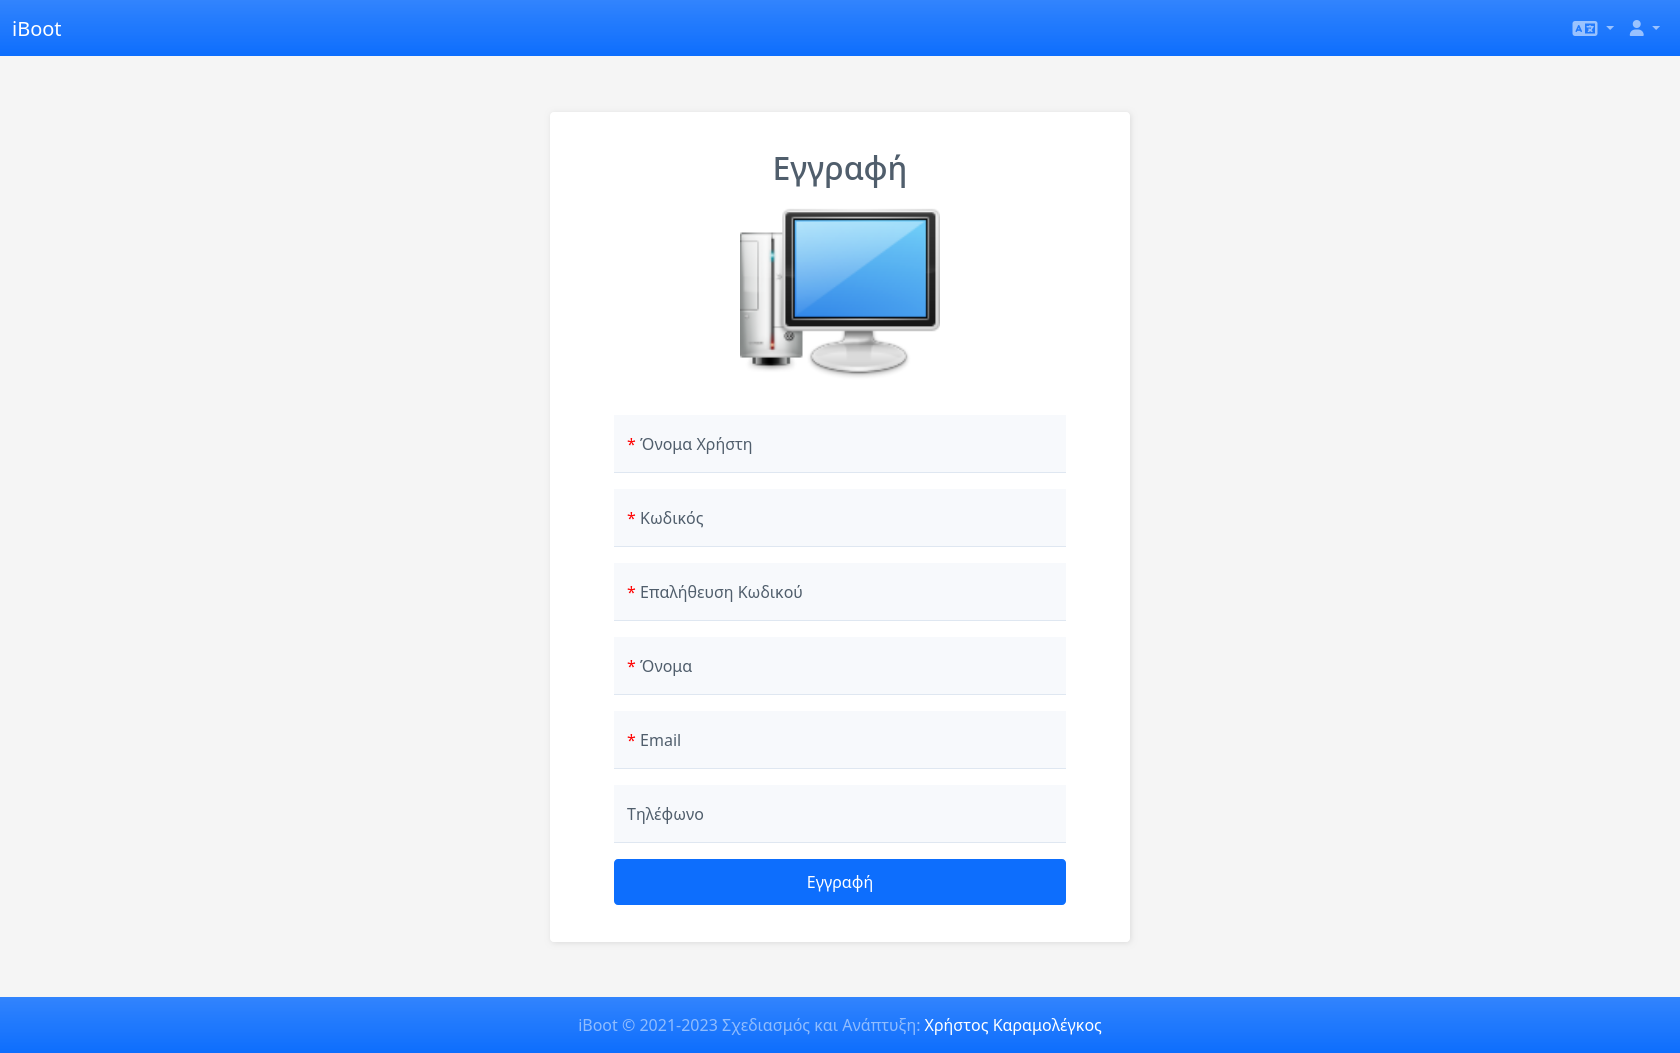
\includegraphics[scale=0.25]{iBoot-register.png}
	\caption{iBoot - Εγγραφή}
	\label{fig:iBoot_register}
\end{figure}

\begin{figure}[ht]
	\centering
	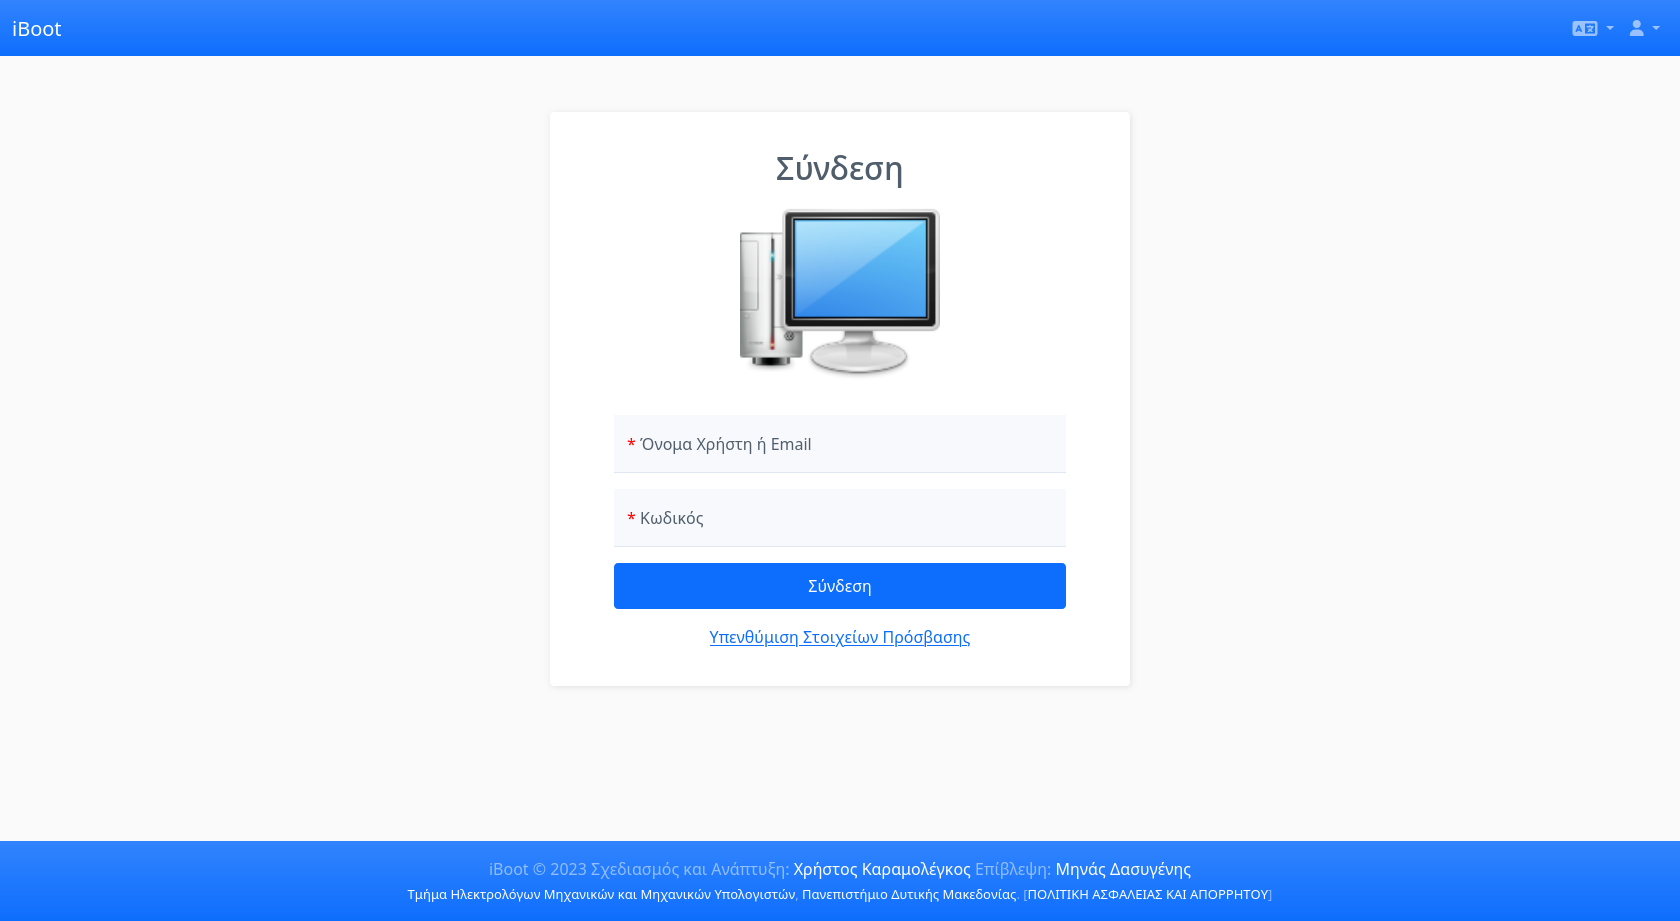
\includegraphics[scale=0.25]{iBoot-login.png}
	\caption{iBoot - Σύνδεση}
	\label{fig:iBoot_login}
\end{figure}

\begin{figure}[ht]
	\centering
	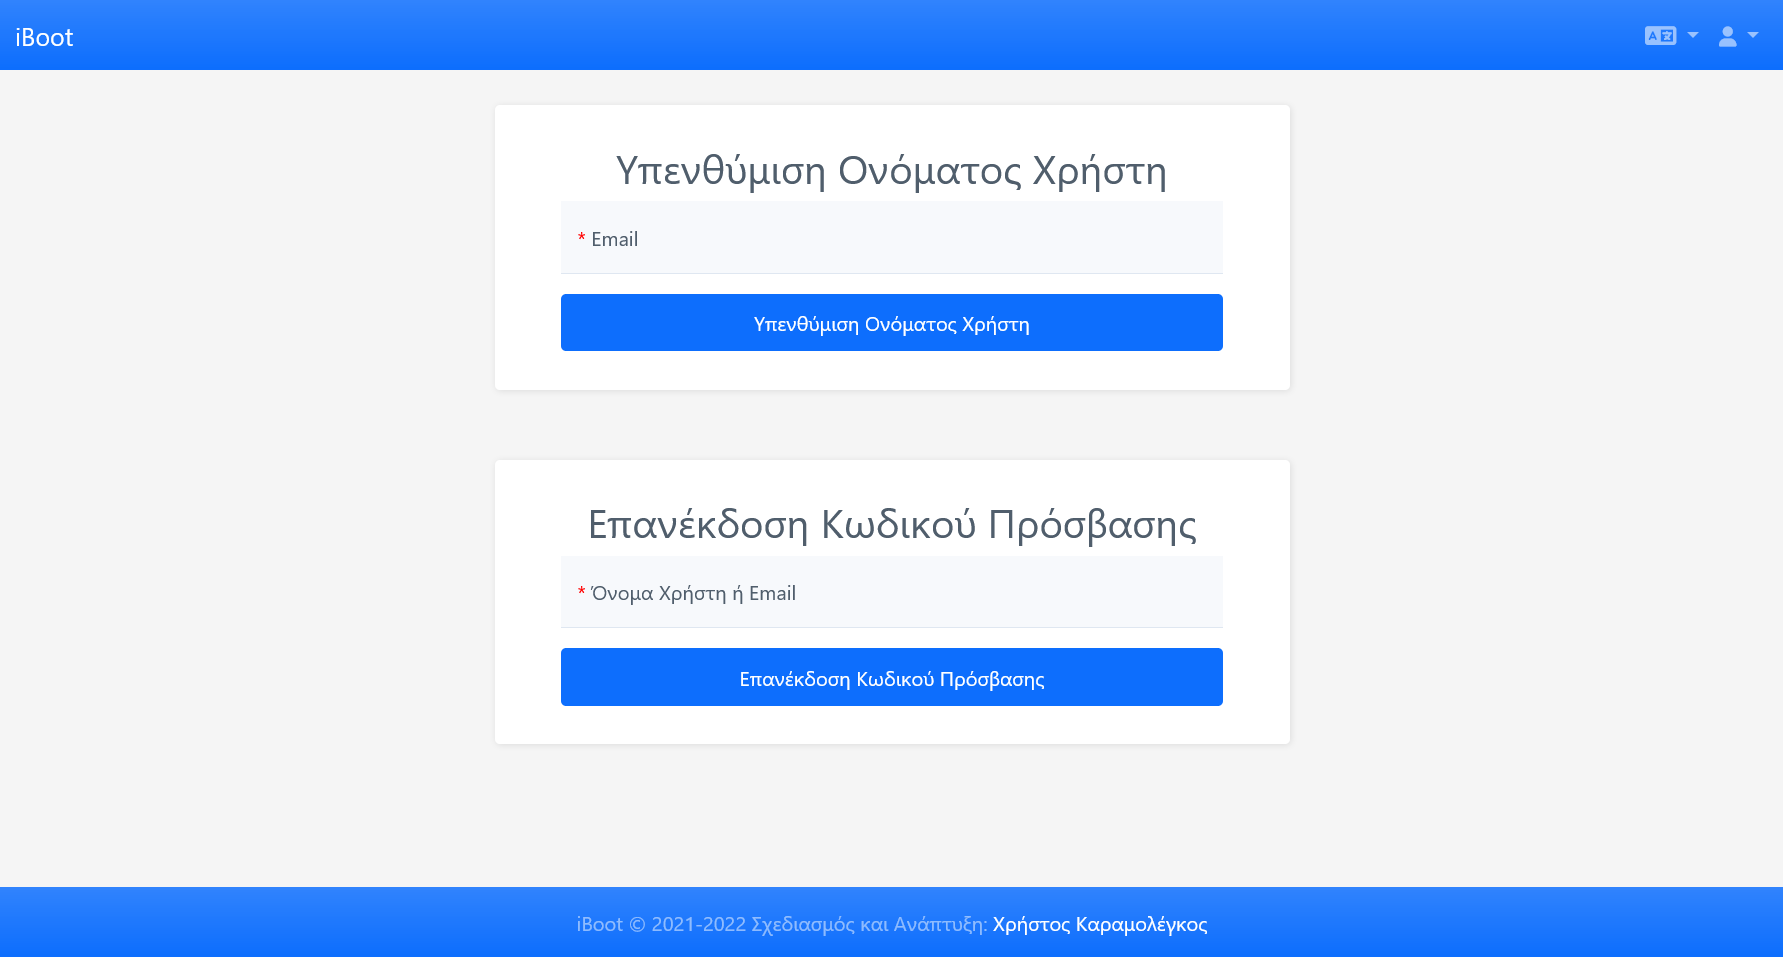
\includegraphics[scale=0.25]{iBoot-forgot-credentials.png}
	\caption{iBoot - Υπενθύμιση Στοιχείων Πρόσβασης}
	\label{fig:iBoot_forgot_credentials}
\end{figure}

\FloatBarrier

\subsection{Μενού Πλοήγησης}

\subsection{Υπολογιστές}

\subsection{Ομάδες Υπολογιστών}

\subsection{Εργαστήρια}

\subsection{Block εντολών τύπου ipxe}

\subsection{Μενού Εκκίνησης}

\subsection{Χρονοδιαγράμματα}

\subsection{Προδιαγραφή API}

\section{Επεξήγηση Αρχείων}

\section{Ασφάλεια Συστήματος}

\section{Σύνοψη Κεφαλαίου 4}
Στο κεφάλαιο 4, εξετάστηκαν όλες οι δυνατότητες της διαδικτυακής εφαρμογής και τα βήματα που πρέπει να ακολουθήσει ένας νέος χρήστης για να τις χρησιμοποιήσει. Επιπλέον, παρασχέθηκε οπτικό υλικό για κάθε λειτουργία στην οποία εμφανιζόταν στον χρήστη η διεπαφή χρήστη της διαδικτυακής εφαρμογής κατά την πλοήγησή του. Στη συνέχεια, εξηγήθηκαν διεξοδικά τόσο το front-end όσο και το back-end της δομής του πληροφοριακού συστήματος. Προκειμένου να διασφαλιστεί η ασφάλεια κατά τη χρήση της διαδικτυακής εφαρμογής, παρέχεται επεξήγηση των πρωτοκόλλων και των προσεγγίσεων ασφαλείας.

Στο επόμενο κεφάλαιο θα γίνει αξιολόγηση του συστήματος, ως προς την ορθή λειτουργία του και τις δυνατότητες κλιμάκωσής του.
